
\section{Diseno del Analizador Semántico}
\subsection{Esquema de Traducción}
\begin{lstlisting}[style=EdT]
0. P' -> @{TSG = creaTS(); DesplG = 0; TS_actual = TSG;
    P.func = false}@ P @{liberaTS(TSG)}@
1. P -> D @{ P$_1$ .func = P.func}@ P$_{1}$
2. P -> F @{ P$_1$ .func = P.func}@ P$_{1}$
3. P -> @{S.func = false}@ S @{P$_1$ = P.func}@ P$_1$
4. D -> var @{zona_decl = true}@ T id ; @{InsertarTipoTS(id.posi, T.tipo)
       							 if(TS_actual=TSG) then
           							 InsertarDespl(id.posi, desplG)
           							 desplG = desplG + T.tamano
      						     else
           							 InsertarDespl(id.posi, desplL)
            						 desplL = desplL + T.tamano
        						zona_decl=false}@
5. T -> int @{T.tipo=entero; T.tamano = 1}@
6. T -> string @{T.tipo=cadena; T.tamano = 64}@
7. T -> boolean @{T.tipo=logico; T.tamano = 1}@
8. F -> function @{zona_decl =true}@ T$_1$ id ( @{TSL = creaTS();desplL=0;
	TS_actual = TSL}@ A )@{InsertaTipoTSG(id.posi,A.tipo -> T.tipo));
    zona_decl = false}@ { @{ C.func = true}@ C } @{if (C.tipoRet != T.tipo)
   											 then error(2);
   											 TS_actual = TSG; LiberarTS(TSL)}@
9. T$_1$ -> λ @{T.tipo = tipo_vacio}@
10. T$_1$ -> T @{T$_1$.tipo = T.tipo}@
11. A -> T id @{InsertarTipoTS(id.posi, T.tipo); InsertarDesplTS(id.posi, desplL);
     desplL = desplL + T.tamano}@ K @{A.tipo = if(K.tipo = tipo_vacio)
                            					then T.tipo
                         					else
                             					T.tipo x K.tipo}@
12. A -> λ @{A.tipo = tipo_vacio}@
13. K -> λ @{K.tipo = tipo_vacio}@
14. K -> , T id @{InsertarTipoTS(id.posi, T.tipo);
	InsertarDesplTS(id.posi, desplL); desplL = desplL + T.tamano}@ K$_1$ 
	@{K.tipo = if(K$_1$.tipo = tipo_vacio)
     				then T.tipo
          		else
            		T.tipo x K.tipo}@
15. C -> D @{C$_1$.func = C.func}@ C$_1$ @{C.tipoRet = C$_1$.tipoRet}@
16. C -> @{S.func = C.func}@ S @{C$_1$.func = C.func}@ C$_1$ @{C.tipoRet =
        								if(S.tipoRet = C$_1$.tipoRet) then
           									S.tipoRet
       									else if(S.tipoRet = tipo_vacio) then
           									C$_1$.tipoRet
        								else if(C$_1$.tipoRet = tipo_vacio) then
           									S.tipoRet
        								else
           									error(2)}@
17. C -> λ @{C.tipoRet = tipo_vacio}@
18. S-> id L E ; @{S.tipo = if(BuscaTipoTS(id.posi) = E.tipo) 
								AND (E.tipo != tipo_error))
								then tipo_ok
     						else
        						error(3)
        					S.tipoRet = tipo_vacio}@
        					
19. S-> id (M); @{S.tipo = if(BuscaTipoTS(id.posi) = M.tipo -> t)
        					then tipo_ok
    					 else
        					error(4)
        				S.tipoRet = tipo_vacio}@
20. S -> print (E); @{S.tipo = if(E.tipo = entero || E.tipo = cadena)
        						then tipo_ok
    						 else
        						error(4)
        					S.tipoRet = tipo_vacio}@
21. S -> input(id); @{S.tipo =
	if(BuscaTipoTS(id.posi) = entero || BuscaTipoTS(id.posi).tipo = cadena))
    	then tipo_ok
    else
    	error(4)
     S.tipoRet = tipo_vacio}@
22. S -> if(E) @{S$_1$.func = S.func}@ S$_1$ @{S.tipo =
    								if(E.tipo = logico) then S$_1$.tipo
    								else
        								error(5)
     								S.tipoRet = S$_1$.tipoRet}@
23. S -> return X; @{S.tipo = if(S.func) then
        						if(X.tipo != tipo.error) then tipo_ok
        						else
           							 error(6)
     						else
        						error(1)
    						 S.tipoRet = X.tipoRet}@
24. L -> |= @{}@
25. L-> = @{}@
26. M-> EQ @{M.tipo =
     if(E.tipo != tipo_error
     AND Q.tipo != tipo_error)
        then if(Q.tipo == tipo_vacio)
                then E.tipo
             else
                E.tipo x Q.tipo
     else
        error(7)}@
27. M -> λ @{M.tipo = tipo_vacio}@
28. Q -> λ @{Q.tipo = tipo_vacio}@
29. Q -> ,EQ$_1$ @{Q.tipo=
                   if(E.tipo != tipo_error
                   AND Q.tipo != tipo_error)
                     then if(Q.tipo == tipo_vacio)
                            then NuevaPila(E.tipo)
                          else Q.tipo.push(E.tipo)
                   else
                     error(7)}@
                     
                     
                     
                     
                     
                     
                     
                     
30. S$_1$ -> { @{S$_2$.func = S$_1$.func}@ S$_2$}
     @{G.func=S$_1$.func}@ G @{S$_1$.tipo =
                            if(S$_2$.tipo != tipo_error)
                                if(G.tipo != tipo_error)
                                    then S$_2$.tipo
                                else error(9)
                            else error(8);
     S$_1$.tipoRet = if (S$_2$.tipoRet = G.tipoRet OR G.tipoRet = tipo_vacio)
						then S$_2$.tipoRet
				else error(10)}@
31. S1 -> @{S$_2$.func=S$_1$.func}@ S @{S$_1$.tipo=S.tipo; S$_1$.tipoRet = S.tipoRet}@
32. G -> else{ @{S$_2$.func=G.func}@ S$_2$}@{G.tipo=S$_2$.tipo; 
						G.tipoRet = S$_2$.tipoRet}@
33. G -> λ @{G.tipo = tipo_vacio; G.tipoRet = tipo_vacio}@
34. X -> E @{X.tipo = E.tipo}@
35. X -> λ @{X.tipo = tipo_vacio}@
36. E -> E$_1$ < U @{E.tipo = if(E$_1$.tipo = U.tipo = entero)
                                then logico
                              else
                                error(11)}@
37. E -> U @{E.tipo = U.tipo}@
38. U -> U$_1$ + R @{U.tipo = if(U$_1$.tipo = R.tipo = entero)
                                then entero
                                else
                                  error(11)}@
39. U-> R @{U.tipo = R.tipo}@
40. R -> !V @{R.tipo = if(V.tipo = logico) then logico
                       else error(11)}@
41. R -> V @{R.tipo = V.tipo}@
42. V -> (E) @{V.tipo = E.tipo}@
43. V -> id @{V.tipo = BuscaTS(id.posi)}@
44. V -> id(M) @{S.tipo = if(BuscaTipoTS(id.posi) = M.tipo -> t)
                            then t
                          else
                            error(4)}@
45. V -> ent @{V.tipo = entero}@
46. V -> cadena @{V.tipo = cadena}@
47. S$_2$ -> @{S.func = S$_2$.func}@ S @{S'$_2$.func = S$_2$.func}@ S'$_2$ @{
              S$_2$.tipo =
                  if(S.tipo != tipo_error) then S$_2$.tipo
                  else
                    error(12);
              S$_2$.tipoRet = if (S.tipoRet =) tipo_vacio) then 
				S'$_2$.tipoRet
			else if (S'$_2$.tipoRet =) tipo_vacio) then
				S.tipoRet
			else error(13) }@
48. S$_2$ -> @{S.func = S$_2$.func}@ S @{S$_2$.tipo = S.tipo; 
					S$_2$.tipoRet = S.tipoRet}@
49. P -> λ @{}@
\end{lstlisting}
\newpage
\subsection{Implementación del EdT}
\begin{lstlisting}[style=EdT]
0. P' -> MM$_{1}$ P @{liberaTS(TSG)}@
1. P -> D P$_{1}$ @{Aux[ntope].tipoRet = Aux[tope].tipoRet}@
2. P -> F P$_{1}$ @{Aux[ntope].tipoRet = Aux[tope].tipoRet}@
3. P -> S P$_{1}$ @{Aux[ntope].tipoRet = if(Aux[tope-1].tipoRet = tipo_vacio)then 
										Aux[tope].tipoRet
								   else error(1)}@
4. D -> var MM$_{2}$ T id MM$_{8}$ ; @{InsertarTipoTS(Aux[tope-2].posi, Aux[tope-3].tipo)
       						 if(TS_actual = TSG) then
           						 InsertarDespl(Aux[tope-1].posi, desplG)
           						 desplG = desplG + Aux[tope-3].tamano
       						 else
           						 InsertarDespl(Aux[tope-2].posi, desplL)
            					 desplL = desplL + Aux[tope-3]}@ 
5. T -> int @{Aux[ntope].tipo=entero; Aux[ntope].tamano = 1}@
6. T -> string @{Aux[ntope].tipo=cadena; Aux[ntope].tamano = 64}@
7. T -> boolean @{Aux[ntope].tipo=logico; Aux[ntope].tamano = 1}@
8. F -> function MM$_{3}$ T$_1$ id MM$_{4}$ ( A ) MM$_{5}$ { C } 
		@{if (Aux[tope-1].tipoRet != Aux[tope-9].tipo)then error(2);
		TS_actual = TSG; LiberarTS(TSL)}@
9. T$_1$ -> λ @{Aux[ntope].tipo = tipo_vacio}@
10. T$_1$ -> T @{Aux[ntope].tipo = Aux[tope].tipo}@
11. A -> T id MM$_{6}$ K @{Aux[ntope].tipo = if(Aux[tope].tipo = tipo_vacio)
										  then Aux[tope-3].tipo}
									   else
										  Aux[tope].tipo.push(Aux[tope-3].tipo)}@
12. A -> λ @{Aux[ntope].tipo = tipo_vacio}@
13. K -> λ @{Aux[ntope].tipo = tipo_vacio}@
14. K -> , T id MM$_{7}$ K$_1$ @{Aux[ntope].tipo = if(Aux[tope].tipo = tipo_vacio)
                    				then NuevaPila(Aux[tope-2].tipo)
             					else
                    				Aux[tope].tipo.push(Aux[tope-4].tipo)}@
15. C -> D C$_1$ @{Aux[ntope].tipoRet = Aux[tope].tipoRet}@           
16. C -> S C$_1$ @{Aux[ntope].tipoRet=
        		if(Aux[tope-1].tipoRet = Aux[tope].tipoRet) then
            		Aux[tope-1].tipoRet
        		else if(Aux[tope-1].tipoRet = tipo_vacio) then
            		Aux[tope-1].tipoRet
        		else if(Aux[tope].tipoRet = tipo_vacio) then
            		Aux[tope-1].tipoRet}
        		else
            		error(2)}@   
17. C -> λ @{Aux[ntope].tipoRet = tipo_vacio}@
18. S-> id L E ; @{Aux[ntope].tipo =
     if(BuscaTipoTS(Aux[tope-3].posi)=(Aux[tope-1].tipo)
    		 AND (Aux[tope-1].tipo != tipo_error))then
        tipo_ok
     else
        error(3)
     Aux[ntope].tipoRet = tipo_vacio}@
19. S-> id (M) ; @{Aux[ntope].tipo =
     if(BuscaTipoTS(Aux[tope-4].posi) = ParFunc(Aux[tope-2].tipo, t)
        then tipo_ok
     else error(4)
     Aux[ntope].tipoRet = tipo_vacio}@
     
     
20. S -> print (E) ; @{Aux[ntope].tipo =
     if(Aux[tope-2].tipo = entero || Aux[tope-2].tipo = cadena)
        then tipo_ok
     else error(4)
     Aux[ntope].tipoRet = tipo_vacio}@
21. S -> input(id); @{Aux[ntope].tipo =
     if(BuscaTipoTS(Aux[tope-2].posi = entero
        || Aux[tope-2].tipo = cadena)) then tipo_ok
     else error(4)
     Aux[ntope].tipoRet = tipo_vacio}@
22. S -> if(E) S$_1$ @{Aux[ntope].tipo =
     if(Aux[tope-2].tipo = logico) then Aux[tope].tipo
     else error(5)
     Aux[ntope].tipoRet = tipo_vacio}@
23. S -> return X ; @{Aux[ntope].tipo =
     if(Aux[tope-1].tipo != tipo.error) then tipo_ok
     else error(6)}@
24. L -> |= @{}@
25. L-> = @{}@
26. M-> EQ @{Aux[ntope].tipo =
     if(Aux[tope-1].tipo != tipo_error
     AND Aux[tope].tipo != tipo_error)
        then if(Aux[tope].tipo = tipo_vacio)
                then Aux[tope-1].tipo
             else
                Aux[tope].tipo.push(Aux[tope-1].tipo)
     else
        error(7)}@
27. M -> λ @{Aux[ntope].tipo = tipo_vacio}@
28. Q -> λ @{Aux[ntope].tipo = tipo_vacio}@
29. Q -> , E Q$_1$ @{if(Aux[tope-1].tipo != tipo_error
                  AND Aux[tope].tipo != tipo_error)
                    then if(Aux[tope].tipo = tipo_vacio)
                            then NuevaPila(Aux[tope-1].tipo)
                         else Aux[tope].tipo.push(Aux[tope-1].tipo)
                  else
                    error(7)}@
30. S$_1$ -> { S$_2$} G @{ Aux[ntope].tipo =
                            if(Aux[tope-2].tipo != tipo_error)
                                if(Aux[tope].tipo != tipo_error)
                                    then Aux[tope-2].tipo
                                else error(9)
                            else error(8);
	Aux[ntope].tipoRet =
		if (Aux[tope-2].tipoRet = Aux[tope].tipoRet 
					OR Aux[tope].tipoRet = tipo_vacio)
			Aux[tope-2].tipoRet
		else 
			error(10)}@
31. S1 -> S @{Aux[ntope].tipo = Aux[tope].tipo;
			Aux[ntope].tipoRet = Aux[tope].tipoRet}@
32. G -> else{S$_2$} @{Aux[ntope].tipo = Aux[tope-1].tipo;
					Aux[ntope].tipoRet = Aux[tope-1].tipoRet}@
33. G -> λ @{Aux[ntope].tipo = tipo_vacio;
			Aux[ntope].tipoRet = tipo_vacio}@
34. X -> E @{Aux[ntope].tipo = Aux[tope].tipo}@
35. X -> λ @{Aux[ntope].tipo = tipo_vacio}@

36. E -> E$_1$ < U @{Aux[ntope].tipo =
                   if(Aux[tope-2].tipo = Aux[tope].tipo = entero)
                        then logico
                   else error(11)}@
37. E -> U @{Aux[ntope].tipo = Aux[tope].tipo}@
38. U -> U$_1$ + R @{Aux[ntope].tipo = 
					if(Aux[tope-2].tipo = Aux[tope-2].tipo = entero)
						then entero 
					else error(11)}@
39. U-> R @{Aux[ntope].tipo = Aux[tope].tipo}@
40. R -> !V @{Aux[ntope].tipo = if(Aux[tope].tipo = logico) then 
									logico
             					else error(11)}@
41. R -> V @{Aux[ntope].tipo = Aux[tope].tipo}@
42. V -> (E) @{Aux[ntope].tipo = Aux[tope-1].tipo}@
43. V -> id @{Aux[ntope].tipo = BuscaTipoTS(Aux[tope].posi)}@
44. V -> id(M) @{Aux[ntope].tipo = 
		if(BuscaTipoTS(Aux[tope-3].posi) = ParFunc(Aux[tope-1].tipo, t)) then t
		else error(4)}@
45. V -> ent @{Aux[ntope].tipo = entero}@
46. V -> cadena @{Aux[ntope].tipo = cadena}@
47. S$_2$ -> S S'$_2$ @{Aux[ntope] = if(Aux[tope-1].tipo != tipo_error) then
								 Aux[tope].tipo
							else 
								error(12);
			Aux[ntope] = if(Aux[tope-1].tipoRet = tipo_vacio) then 
							Aux[tope].tipoRet
						else if(Aux[tope].tipoRet = tipo_vacio) then 
							Aux[tope-1].tipoRet 
						else error(13);}@
48. S$_2$ -> S @{Aux[ntope].tipo = Aux[tope].tipo;
			Aux[ntope].tipoRet = Aux[tope].tipoRet}@
49. P -> λ @{Aux[ntope].tipoRet = tipo_vacio}@
50. MM$_{1}$ -> λ @{TSG = creaTS();
			desplG = 0;
			TSA = TSG}@
51. MM$_{2}$ -> λ @{zona_decl = true}@
52. MM$_{3}$ -> λ @{zona_decl = true}@
53. MM$_{4}$ -> λ @{TSL = creaTS();
			desplL = 0;
			TSA = TSL}@
54. MM$_{5}$ -> λ @{InsertarTipoTS(Aux[tope-4].posi, Aux[tope-1].tipo) ;
	InsertarNArgsTS(Aux[tope-4].posi, Aux[tope-1].NArgs) ;
	for i in NArgs :
	InsertarTipoArgsTS(Aux[tope-4].posi, Aux[tope-1].tipoLista(i));
	InsertarEtiquetaTS(Aux[tope-4].posi, Aux[tope-4].lexema + Aux[tope-4].posi); 
	InsertarTipoDevueltoTS(Aux[tope-4].posi, Aux[tope-5].tipo)}@
55. MM$_{6}$ -> λ @{InsertarTipoTS(Aux[tope].posi, Aux[tope-1].tipo) ;
     InsertarDesplTS(Aux[tope].posi, desplL);
     desplL = desplL + Aux[tope-1].tamano}@
56. MM$_{7}$ -> λ @{InsertarTipoTS(Aux[tope].posi, Aux[tope-1].tipo) ;
     InsertarDesplTS(Aux[tope].posi, desplL);
     desplL = desplL + Aux[tope-1].tamano}@
57. MM$_{8}$ -> λ @{zona_decl = false}@
\end{lstlisting}
\newpage
De forma que hemos tenido que transformar el EdT para que en vez de usar atributos heredados, lo cual complica bastante la implementación, hemos transformado el atributo heredado func al atributo sintetizado tipoRet.

También hemos tenido que modificar la gramática del sintáctico añadiendo los marcadores MM$_i$ y sus correspondientes reglas lambda para poder implementar las acciones con efectos laterales.

\begin{lstlisting}[style=EdT]
Ej:
D -> var @{zdecl:=true}@ T id; @{otras acciones}@
Lo transformamos en:
D -> var MM T id; @{otras acciones}@
MM -> lambda @{zdecl:=true}@
\end{lstlisting}

\subsection{Gramática y Autómata Final del A. Sintáctico}
\begin{lstlisting}[style=Gramatica]
Terminales = { ; { } id ent cadena ( ) + < ! = |= var int
	boolean string print input , return function if else }
NoTerminales = { P1 P D T F T1 A K C S L M Q S1 G X E U R V
	S2 M1 M2 M3 M4 M5 M6 M7 M8 }
Axioma = P1
Producciones = {
P1 -> M1 P
P -> D P
P -> F P
P -> S P
D -> var M2 T id M8 ;
T -> int
T -> string
T -> boolean
F -> function M3 T1 id M4 ( A ) M5 { C }
T1 -> lambda
T1 -> T
A -> T id M6 K
A -> lambda
K -> lambda
K -> , T id M7 K
C -> D C
C -> S C
C -> lambda
S -> id L E ;
S -> id ( M ) ;
S -> print ( E ) ;
S -> input ( id ) ;
S -> if ( E ) S1
S -> return X ;
L -> |=
L -> =
M -> E Q
M -> lambda
Q -> lambda
Q -> , E Q
S1 -> { S2 } G
S1 -> S
G -> else { S2 }
G -> lambda
X -> E
X -> lambda
E -> E < U
E -> U
U -> U + R
U -> R
R -> ! V
R -> V
V -> ( E )
V -> id
V -> id ( M )
V -> ent
V -> cadena
S2 -> S S2
S2 -> S
P -> lambda
M1 -> lambda
M2 -> lambda
M3 -> lambda
M4 -> lambda
M5 -> lambda
M6 -> lambda
M7 -> lambda
M8 -> lambda
}
\end{lstlisting}
Dando lugar a modificaciones en el Autómata (y en consecuencia en la Tabla de Decisión):
\begin{lstlisting}[style =EstadosAutomataST]
Donde:
S$_{-1}$={P2 ->  . P1, P1 -> . MM1 P, P -> . SP, MM1 -> .}
S$_{1}$={P1 -> MM1 P .} [Ahora no se ACEPTA, solo se REDUCE]
S$_{100}$={P2 -> P1 .} [Ahora este es el estado que ACEPTA]
S$_{101}$={D -> var .  MM2 T id MM8 ;, MM2 -> .}
S$_{102}$={F -> function . MM3 T1 id MM4 ( A ) MM5 { C }, MM3 -> .}
S$_{103}$={F -> function MM3 T1 id . MM4 ( A ) MM5 { C }, MM4 -> .}
S$_{104}$={D -> F -> function .  MM3 T1 id MM4 ( A ) . MM5 { C }, MM5 -> .}
S$_{105}$={A -> T id . MM6 K, MM6 -> .}
S$_{106}$={D -> , T id . MM7 K, MM7 -> .}
S$_{107}$={D -> var MM2 T id . MM8 ;, MM8 -> .}
\end{lstlisting}
\newpage
\mbox{}
\begin{textblock}{1}(0.5,1)
\centering
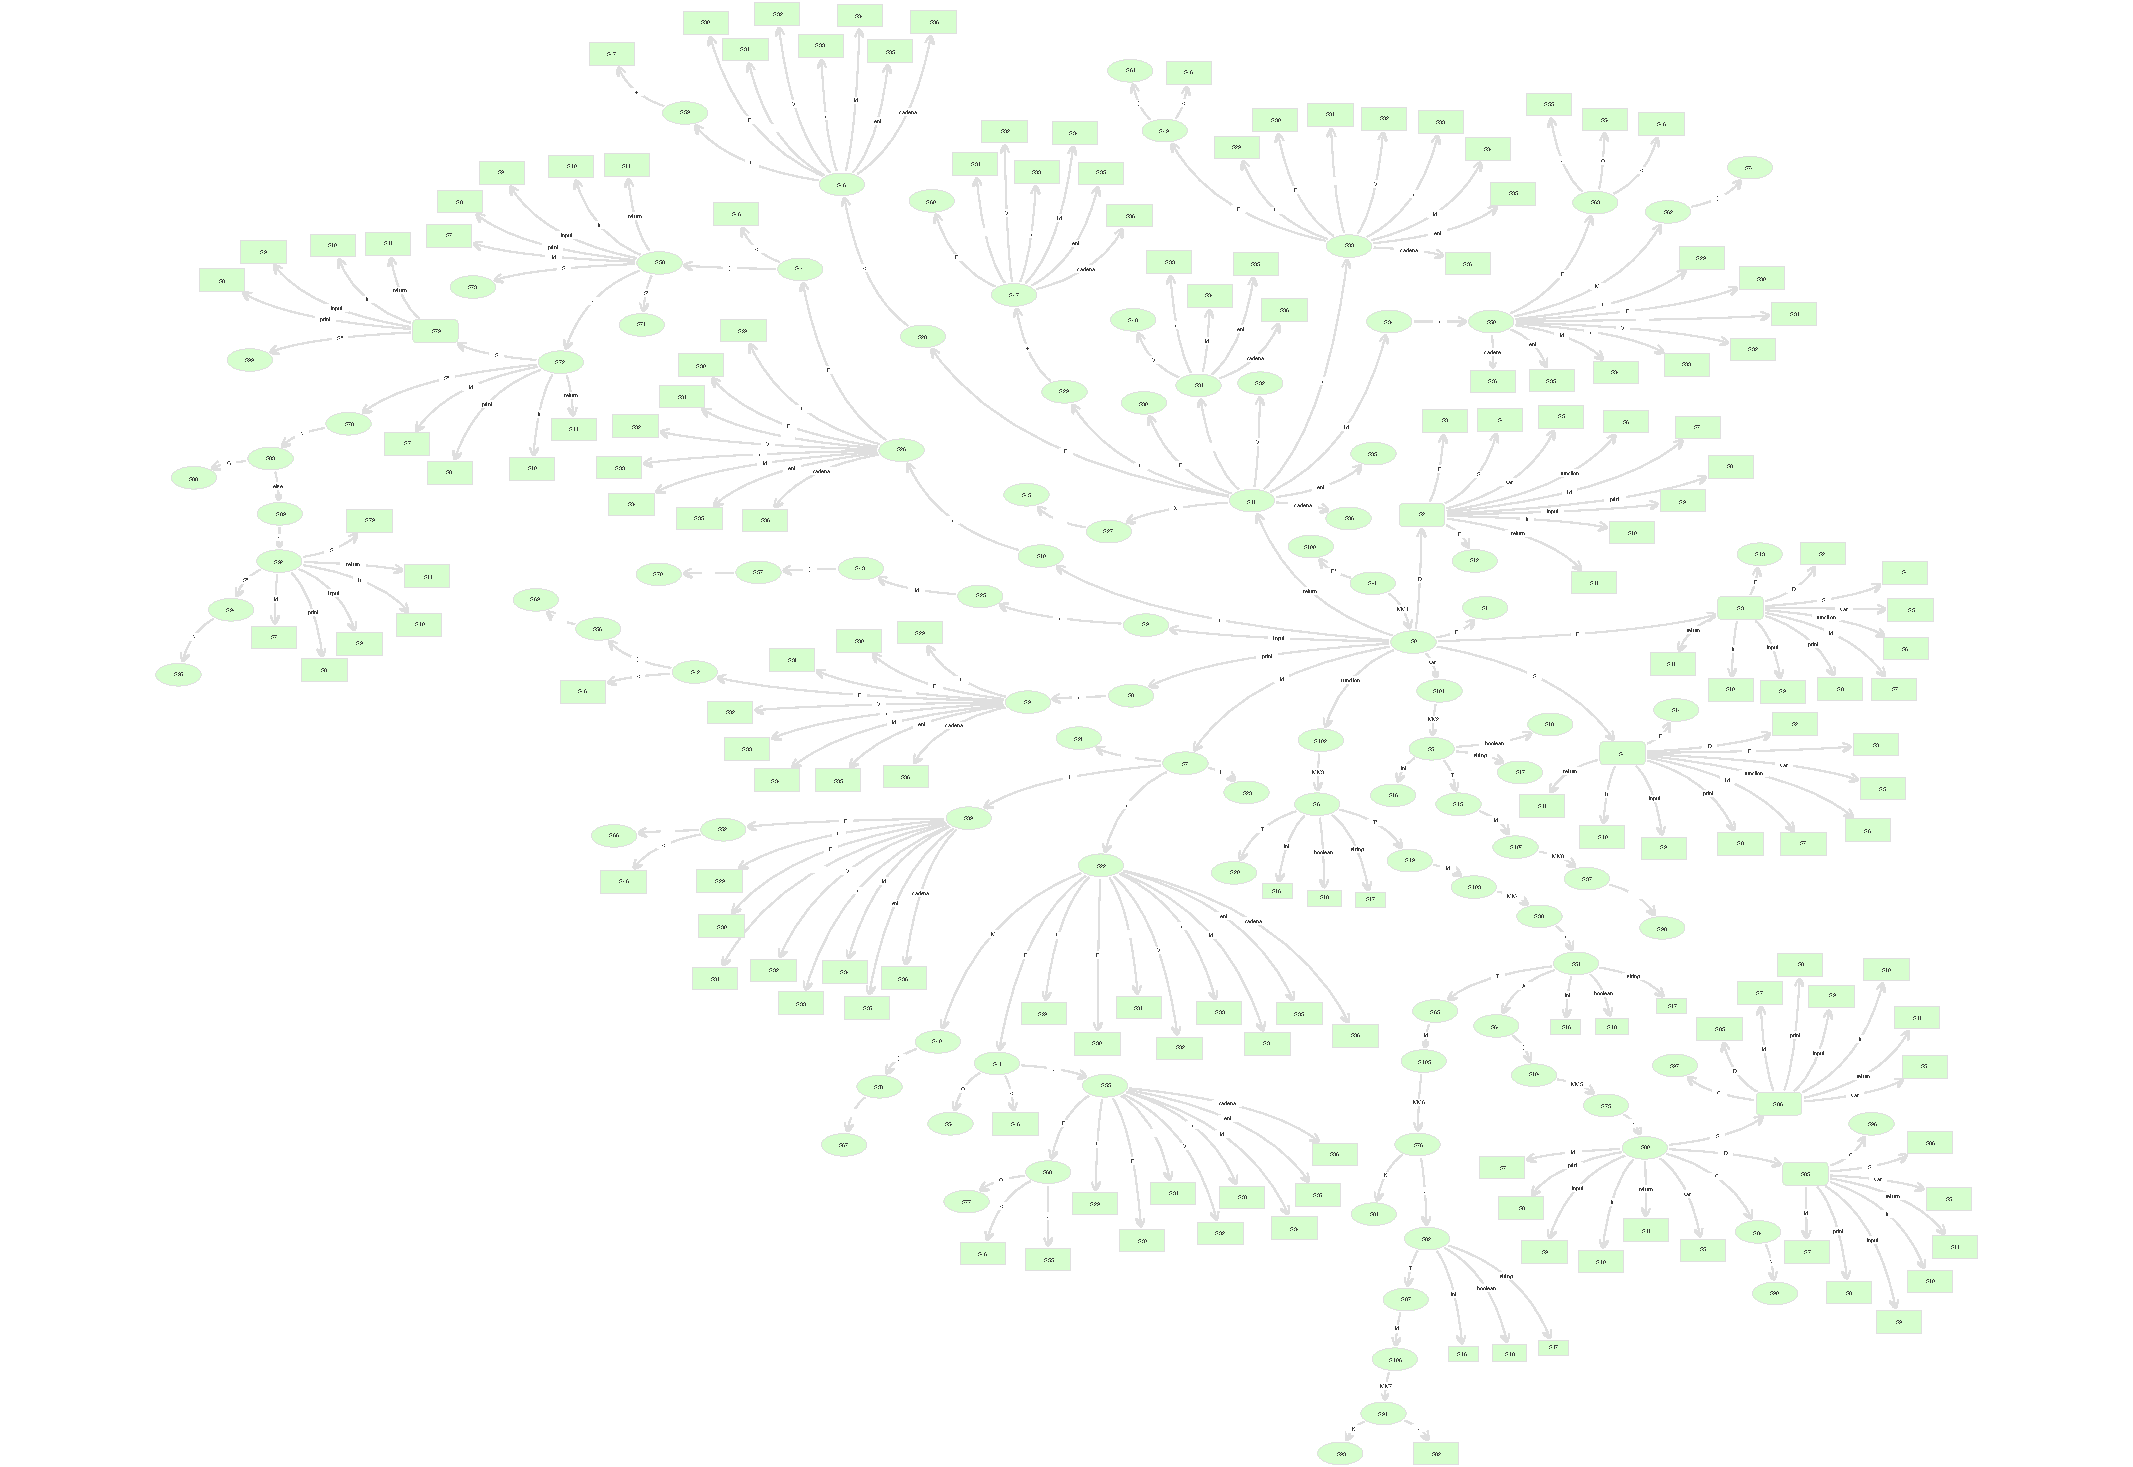
\includegraphics[width=20cm]{Enrico.pdf}
\end{textblock}
\begin{textblock}{14}(2,8.5)
\subsection{Errores}

\noindent Error 1: "RETURN fuera de funcion."\\
\noindent Error 2: "El tipo devuelto no coincide con el declarado en la funcion."\\
\noindent Error 3: "Asignacion incorrecta.";\\
\noindent Error 4: "Incoherencia entre parametros formales y actuales en la llamada a funcion.";\\
\noindent Error 5: "La condicion del IF no es de tipo logico.";\\
\noindent Error 6: "Error en la sentencia del RETURN.";\\
\noindent Error 7: "Error al definir los parametros de llamada de una funcion.";\\
\noindent Error 8: "Error en el cuerpo del IF.";\\
\noindent Error 9: "Error en el cuerpo del ELSE.";\\
\noindent Error 10: "No concuerdan los RETURN de las sentencias IF-ELSE.";\\
\noindent Error 11: "Tipos incompatibles entre operandos y operadores.";\\
\noindent Error 12: "Error en el cuerpo del IF-ELSE.";\\
\noindent Error 13: "Error en el RETURN en el cuerpo del IF-ELSE.";\\
\end{textblock}
